\section{Párování}
\subsection{Definice}
Je dán neorientovaný graf $G = (V,E, \eps)$. Podmnožina hran $P \subseteq E$ se nazývá \ii{párování}, jestliže v $P$ 
neexistují 2 různé hrany se společným krajním vrcholem (takže vrchol má stupeň max. 1).

\subsection{Vrchol nasycený a volný v párování}
Mějme párování $P$. Vrchol $v$ grafu nazvěme \ii{nasycený} v $P$, pokud existuje hrana $e \in P$ incidentní s $v$.

V opačném případě říkáme, že vrchol $v$ je \ii{volný} v $P$.
\begin{figure}[H]
    \centering
    \begin{tikzpicture}[
        red_node/.style={circle, draw=red!70, line width=2pt, fill=red!70, minimum size=1mm, inner sep=0pt},
        blue_node/.style={circle, draw=blue!60, line width=2pt, fill=blue!60, minimum size=1mm, inner sep=0pt},
        purple_node/.style={circle, draw=purple, line width=2pt, fill=purple, minimum size=1mm, inner sep=0pt},
        edge_style/.style={draw=black, line width=1pt, line cap=round}
    ]

        \node[red_node] (r_bot_1) at (0, 0) {};
        \node[red_node] (r_bot_2) at (2, 0) {};
        \node[red_node] (r_bot_3) at (4, 0) {};

        \node[red_node] (r_top_1) at (0, 2.5) {};
        \node[red_node] (r_top_2) at (2, 2.5) {};
        \node[red_node] (r_top_3) at (4, 2.5) {};

        \node[blue_node] (b_left)  at (-1, 3.5) {};
        \node[blue_node] (b_right) at (5, -1.0) {};


        \draw[edge_style] (r_bot_1) -- (r_bot_2) -- (r_bot_3);
        \draw[edge_style] (r_top_1) -- (r_top_2) -- (r_top_3);

        \draw[edge_style] (r_bot_1) -- (r_top_1);
        \draw[edge_style] (r_bot_2) -- (r_top_2);
        \draw[edge_style] (r_bot_3) -- (r_top_3);

        \draw[draw=purple, line width=1pt, line cap=round, decoration={snake, amplitude=.4mm}, decorate] (r_bot_1) -- (r_top_1);
        \draw[draw=purple, line width=1pt, line cap=round, decoration={snake, amplitude=.4mm}, decorate] (r_bot_2) -- (r_top_2);
        \draw[draw=purple, line width=1pt, line cap=round, decoration={snake, amplitude=.4mm}, decorate] (r_bot_3) -- (r_top_3);

        \draw[edge_style] (r_bot_1) -- (r_top_2);
        \draw[edge_style] (r_bot_2) -- (r_top_3);

        \draw[edge_style] (b_left) -- (r_top_1);
        \draw[edge_style] (b_right) -- (r_bot_3);

        \matrix [
            % draw=white,
            % fill=white,
            line width=1pt,
            rounded corners=0pt,
            inner sep=2pt,
            row sep=1pt,
            column sep=5pt,
            right=0.5cm of r_top_3,
            anchor=north west
        ] {
            \node[red_node, scale=0.7] {}; & \node[anchor=west] {nasycený}; \\
            \node[blue_node, scale=0.7] {}; & \node[anchor=west] {volný}; \\
            \node[minimum width=0.6cm] (p_line) {}; 
                \draw[purple, line width=1pt, decoration={snake, amplitude=.3mm, segment length=1.5mm}, decorate] (p_line.west) -- (p_line.east); 
                & \node[anchor=west, font=\small] {párování $P$}; \\
        };
    \end{tikzpicture}
\end{figure}

\subsection{Perfektní párování}
Párování $P$ v grafu $G$ nazveme \ii{perfektní párování}, jestliže každý vrchol grafu je nasycen v $P$. To znamená, že 
$P$ má $\frac{n}{2}$ hran, kde $n$ je počet vrcholů grafu $G$.

\subsection{Maximální párování}
Párování $P$ v grafu $G$ nazveme \ii{maximální párování}, jestliže je nejpočetnější mezi všemi párováními v grafu $G$.

Perfektní párování je jistě maximální. Naopak to neplatí. Existují grafy, které perfektní párování nemají --- stačí 
uvažovat grafy s lichým počtem vrcholů. Ovšem ani grafy se sudým počtem vrcholů nemusí perfektní párování obsahovat.

V každém grafu existuje maximální párování. 

\subsection{Střídavá cesta vůči párování \texorpdfstring{$P$}{P}}
Je dáno párování $P$ v grafu $G$. Cesta $C = e_1, e_2, \dots, e_k$ v grafu $G$ se nazývá \ii{střídavá cesta vůči $P$}, 
jestliže platí následující dvě podmínky:
\begin{enumerate}[1)]
    \item hrany z cesty $C$ střídavě leží a neleží v párování $P$,
    \item jestliže krajní vrchol $v$ cesty $C$ je nasycen v $P$, pak $C$ obsahuje i hranu párování $P$, která vrchol $v$ 
    nasycuje.
\end{enumerate}
\begin{figure}[H]
    \centering
    \begin{tikzpicture}[
        red_node/.style={circle, draw=red!70, line width=2pt, fill=red!70, minimum size=1mm, inner sep=0pt},
        blue_node/.style={circle, draw=blue!60, line width=2pt, fill=blue!60, minimum size=1mm, inner sep=0pt},
        purple_node/.style={circle, draw=purple, line width=2pt, fill=purple, minimum size=1mm, inner sep=0pt},
        green_node/.style={circle, draw=green!70!black, line width=2pt, fill=green!70!black, minimum size=1mm, inner sep=0pt},
        edge_style/.style={draw=black, line width=1pt, line cap=round},
        yellow_edge/.style={draw=green!70!black, line width=1pt, line cap=round}
    ]

        \node[red_node] (r_bot_1) at (0, 0) {};
        \node[red_node] (r_bot_2) at (2, 0) {};
        \node[red_node] (r_bot_3) at (4, 0) {};

        \node[red_node] (r_top_1) at (0, 2.5) {};
        \node[red_node] (r_top_2) at (2, 2.5) {};
        \node[red_node] (r_top_3) at (4, 2.5) {};

        \node[blue_node] (b_left)  at (-1, 3.5) {};
        \node[blue_node] (b_right) at (5, -1.0) {};


        \draw[edge_style] (r_bot_1) -- (r_bot_2) -- (r_bot_3);
        \draw[edge_style] (r_top_1) -- (r_top_2) -- (r_top_3);

        \draw[yellow_edge] (r_bot_1) -- (r_top_1);
        \draw[yellow_edge] (r_bot_2) -- (r_top_2);
        \draw[yellow_edge] (r_bot_3) -- (r_top_3);

        \draw[draw=purple, line width=1pt, line cap=round, decoration={snake, amplitude=.4mm}, decorate] (r_bot_1) -- (r_top_1);
        \draw[draw=purple, line width=1pt, line cap=round, decoration={snake, amplitude=.4mm}, decorate] (r_bot_2) -- (r_top_2);
        \draw[draw=purple, line width=1pt, line cap=round, decoration={snake, amplitude=.4mm}, decorate] (r_bot_3) -- (r_top_3);

        \draw[yellow_edge] (r_bot_1) -- (r_top_2);
        \draw[yellow_edge] (r_bot_2) -- (r_top_3);

        \draw[yellow_edge] (b_left) -- (r_top_1);
        \draw[yellow_edge] (b_right) -- (r_bot_3);

        \matrix [
            % draw=white,
            % fill=white,
            line width=1pt,
            rounded corners=0pt,
            inner sep=2pt,
            row sep=1pt,
            column sep=5pt,
            right=0.5cm of r_top_3,
            anchor=north west
        ] {
            \node[red_node, scale=0.7] {}; & \node[anchor=west] {nasycený}; \\
            \node[blue_node, scale=0.7] {}; & \node[anchor=west] {volný}; \\
            \node[minimum width=0.6cm] (p_line) {}; 
                \draw[purple, line width=1pt, decoration={snake, amplitude=.3mm, segment length=1.5mm}, decorate] (p_line.west) -- (p_line.east); 
                & \node[anchor=west, font=\small] {párování $P$}; \\
            \node[minimum width=0.6cm] (g_line) {}; 
                \draw[green!70!black, line width=1pt] (g_line.west) -- (g_line.east); 
                & \node[anchor=west, font=\small] {cesta $C$}; \\
        };
    \end{tikzpicture}
\end{figure}

\subsection{Zlepšující cesta vůči párování \texorpdfstring{$P$}{P}}
Střídavá cesta mezi volnými vrcholy se nazývá \ii{zlepšující cesta vůči $P$}.

\subsection{Tvrzení o střídavé cestě}
Jestliže $C$ je střídavá cesta vůči párování $P$, pak množina hran $P^\prime = C \oplus P$ je také párování v $G$.
\ii{Připomeňme, že symetrická diference $A \oplus B$ dvou množin $A, B$ je množina
\begin{equation}
    A \oplus B = (A \cup B) \setminus (A \cap B) = (A \setminus B) \cup (B \setminus A).
\end{equation}
}
\begin{figure}[H]
    \centering
    \begin{minipage}[c]{0.42\textwidth}
            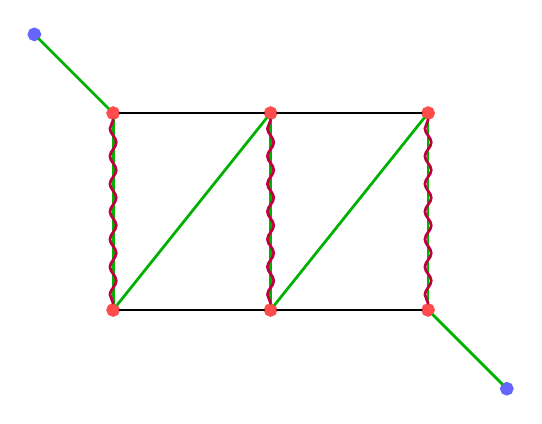
\begin{tikzpicture}[
                red_node/.style={circle, draw=red!70, line width=2pt, fill=red!70, minimum size=1mm, inner sep=0pt},
                blue_node/.style={circle, draw=blue!60, line width=2pt, fill=blue!60, minimum size=1mm, inner sep=0pt},
                purple_node/.style={circle, draw=purple, line width=2pt, fill=purple, minimum size=1mm, inner sep=0pt},
                green_node/.style={circle, draw=green!70!black, line width=2pt, fill=green!70!black, minimum size=1mm, inner sep=0pt},
                edge_style/.style={draw=black, line width=1pt, line cap=round},
                yellow_edge/.style={draw=green!70!black, line width=1pt, line cap=round}
            ]

                \node[red_node] (r_bot_1) at (0, 0) {};
                \node[red_node] (r_bot_2) at (2, 0) {};
                \node[red_node] (r_bot_3) at (4, 0) {};

                \node[red_node] (r_top_1) at (0, 2.5) {};
                \node[red_node] (r_top_2) at (2, 2.5) {};
                \node[red_node] (r_top_3) at (4, 2.5) {};

                \node[blue_node] (b_left)  at (-1, 3.5) {};
                \node[blue_node] (b_right) at (5, -1.0) {};


                \draw[edge_style] (r_bot_1) -- (r_bot_2) -- (r_bot_3);
                \draw[edge_style] (r_top_1) -- (r_top_2) -- (r_top_3);

                \draw[yellow_edge] (r_bot_1) -- (r_top_1);
                \draw[yellow_edge] (r_bot_2) -- (r_top_2);
                \draw[yellow_edge] (r_bot_3) -- (r_top_3);

                \draw[draw=purple, line width=1pt, line cap=round, decoration={snake, amplitude=.4mm}, decorate] (r_bot_1) -- (r_top_1);
                \draw[draw=purple, line width=1pt, line cap=round, decoration={snake, amplitude=.4mm}, decorate] (r_bot_2) -- (r_top_2);
                \draw[draw=purple, line width=1pt, line cap=round, decoration={snake, amplitude=.4mm}, decorate] (r_bot_3) -- (r_top_3);

                \draw[yellow_edge] (r_bot_1) -- (r_top_2);
                \draw[yellow_edge] (r_bot_2) -- (r_top_3);

                \draw[yellow_edge] (b_left) -- (r_top_1);
                \draw[yellow_edge] (b_right) -- (r_bot_3);
            \end{tikzpicture}
    \end{minipage}%
    \begin{minipage}[c]{0.55\textwidth}
            \begin{tikzpicture}[
                red_node/.style={circle, draw=red!70, line width=2pt, fill=red!70, minimum size=1mm, inner sep=0pt},
                blue_node/.style={circle, draw=blue!60, line width=2pt, fill=blue!60, minimum size=1mm, inner sep=0pt},
                purple_node/.style={circle, draw=purple, line width=2pt, fill=purple, minimum size=1mm, inner sep=0pt},
                green_node/.style={circle, draw=green!70!black, line width=2pt, fill=green!70!black, minimum size=1mm, inner sep=0pt},
                cyan_node/.style={circle, draw=cyan!90!black, line width=2pt, fill=green!70!black, minimum size=1mm, inner sep=0pt},
                edge_style/.style={draw=black, line width=1pt, line cap=round},
                cyan_edge/.style={draw=cyan!90!black, line width=1pt, line cap=round}
            ]

                \node[red_node] (r_bot_1) at (0, 0) {};
                \node[red_node] (r_bot_2) at (2, 0) {};
                \node[red_node] (r_bot_3) at (4, 0) {};

                \node[red_node] (r_top_1) at (0, 2.5) {};
                \node[red_node] (r_top_2) at (2, 2.5) {};
                \node[red_node] (r_top_3) at (4, 2.5) {};

                \node[blue_node] (b_left)  at (-1, 3.5) {};
                \node[blue_node] (b_right) at (5, -1.0) {};


                \draw[edge_style] (r_bot_1) -- (r_bot_2) -- (r_bot_3);
                \draw[edge_style] (r_top_1) -- (r_top_2) -- (r_top_3);

                \draw[edge_style] (r_bot_1) -- (r_top_1);
                \draw[edge_style] (r_bot_2) -- (r_top_2);
                \draw[edge_style] (r_bot_3) -- (r_top_3);

                \draw[cyan_edge] (r_bot_1) -- (r_top_2);
                \draw[cyan_edge] (r_bot_2) -- (r_top_3);

                \draw[cyan_edge] (b_left) -- (r_top_1);
                \draw[cyan_edge] (b_right) -- (r_bot_3);

                \matrix [
                    % draw=white,
                    % fill=white,
                    line width=1pt,
                    rounded corners=0pt,
                    inner sep=2pt,
                    row sep=1pt,
                    column sep=6pt,
                    right=0.5cm of r_top_3,
                    anchor=north west
                ] {
                    \node[red_node, scale=0.7] {}; & \node[anchor=west] {nasycený}; \\
                    \node[blue_node, scale=0.7] {}; & \node[anchor=west] {volný}; \\
                    \node[minimum width=0.6cm] (p_line) {}; 
                    \draw[purple, line width=1pt, decoration={snake, amplitude=.3mm, segment length=1.5mm}, decorate] (p_line.west) -- (p_line.east); 
                        & \node[anchor=west, font=\small] {párování $P$}; \\
                    \node[minimum width=0.6cm] (g_line) {}; 
                        \draw[green!70!black, line width=1pt] (g_line.west) -- (g_line.east); 
                        & \node[anchor=west, font=\small] {cesta $C$}; \\
                    \node[minimum width=0.6cm] (c_line) {}; 
                        \draw[cyan!90!black, line width=1pt] (c_line.west) -- (c_line.east); 
                        & \node[anchor=west, font=\small] {párování $P^\prime$}; \\
                };
            \end{tikzpicture}
    \end{minipage}
\end{figure}
A pokud je navíc $C$ zlepšující cesta, tj. cesta mezi volnými vrcholy v $P$, pak $|P^\prime| = |P| + 1$.

\subsection{Věta o vrcholově disjunktních zlepšujících cestách}
\ii{Berge}. Je dáno párování $P$ v grafu $G$. Označme $P_{\max}$ maximální párování v $G$ (o kterém víme, že 
existuje). Jestliže
\begin{equation}
    |P_{\max}| = |P| + k,
\end{equation}
pak v $G$ existuje $k$ vrcholově disjunktních zlepšujících cest vůči $P$.

Přitom alespoň jedna z těchto cest je kratší než $\frac{n}{k}$, kde $n$ je počet vrcholů.

\dukaz $H = P \oplus P_{\max} = (P \setminus P_{\max}) \cup (P_{\max} \setminus P)$
% TODO: dodělat důkaz

\subsection{Souvislost perfektního párování a počtu komponent}
\ii{Tutte}. Je dán prostý graf $G = (V,E)$ bez smyček s alespoň třemi vrcholy. V grafu $G$ existuje perfektní párování
právě tehdy, když pro každou podmnožinu $S \subseteq V$ platí
\begin{equation}
    g(G \setminus S) \leq |S|,
\end{equation}
kde $g(G \setminus S)$ je počet komponent souvislosti grafu $G \setminus S$, které mají lichý počet vrcholů.

\dukaz\\
\enquote{$\Rightarrow$}: Předpokládejme, že v grafu $G$ existuje perfektní párování (tj. párování nasycující všechny 
vrcholy grafu $G$). Vezměme libovolnou $S \subseteq V$. Protože v každé liché komponentě souvislosti grafu 
$G \setminus S$ je alespoň jeden vrchol, který není spárován uvnitř komponenty, musí být v perfektním párování spárován
s nějakým vrcholem $S$. Proto nemůže být $|S|$ menší než počet lichých komponent.

\enquote{$\Leftarrow$}: Předpokládejme, že graf $G$ splňuje $g(G \setminus S) \leq |S|$ pro každou $S \subseteq V$.
% TODO: dodělat důkaz

\subsection{Párování v bipartitních grafech}
Je dán bipartitní graf $G$ se stranami $X$ a $Y$. K němu je možné vytvořit síť takovou, že každému párování $P$ v grafu 
$G$ odpovídá přípustný tok $f$, a naopak každému přípustnému toku $f$ v síti odpovídá párování $P$ v $G$; a to tak, že 
$\vel(f) = |P|$.
\begin{figure}[H]
    \centering
    \begin{tikzpicture}[
        vertex/.style={circle, draw, fill=white, inner sep=1pt, outer sep=0pt},
        blue_arrow/.style={->, >=Stealth, blue!70!black, thick},
        black_arrow/.style={->, >=Stealth, black, thick},
        highlight/.style={line width=7pt, yellow!50, line cap=round},
        dashed_line/.style={dotted, black!70, thick}
    ]
        \node[vertex, label=below:$s$] (s) at (0, 0) {};
        \node[vertex, label=below:$t$] (t) at (10, 0) {};

        \def\xpos{3}
        \def\ypos{7}

        \draw[dashed_line] (\xpos, 2.5) -- (\xpos, -2.5);
        \draw[dashed_line] (\ypos, 2.5) -- (\ypos, -2.5);

        \node[vertex] (x1) at (\xpos, 2.5) {};
        \node[vertex] (x2) at (\xpos, 1.2) {};
        \node[vertex] (x3) at (\xpos, -1.2) {};
        \node[vertex] (x4) at (\xpos, -2.5) {};

        \node[vertex] (y1) at (\ypos, 2.5) {};
        \node[vertex] (y2) at (\ypos, 1.2) {};
        \node[vertex] (y3) at (\ypos, -1.2) {};
        \node[vertex] (y4) at (\ypos, -2.5) {};

        \node[above=0.3cm of x1] {$X$};
        \node[above=0.3cm of y1] {$Y$};

        \begin{scope}[on background layer]
            \draw[highlight] (x1) -- (y1);
            \draw[highlight] (x2) -- (y2);
            \draw[highlight] (x3) -- (y4);
            \draw[highlight] (x4) -- (y3);
        \end{scope}

        \draw[blue_arrow] (s) -- (x1);
        \draw[blue_arrow] (s) -- (x2);
        \draw[blue_arrow] (s) -- (x3);
        \draw[blue_arrow] (s) -- (x4);
        \node[blue!70!black, font=\large] at (1.5, 0.2) {$\vdots$};
        \draw[blue_arrow] (y1) -- (t);
        \draw[blue_arrow] (y2) -- (t);
        \draw[blue_arrow] (y3) -- (t);
        \draw[blue_arrow] (y4) -- (t);
        \node[blue!70!black, font=\large] at (8.5, 0.2) {$\vdots$};

        \draw[black_arrow] (x1) -- (y1);
        \draw[black_arrow] (x2) -- (y2);
        \draw[black_arrow] (x3) -- (y4);
        \draw[black_arrow] (x4) -- (y3);
        \draw[black_arrow] (x1) -- (y2);
        \draw[black_arrow] (x2) -- (y1);
        \draw[black_arrow] (x3) -- (y3);
        \draw[black_arrow] (x2) -- (y4);
        \draw[black_arrow] (x4) -- (y2);
    \end{tikzpicture}
\end{figure}
Vytvořme síť $G^\prime$ s omezeními $l,c$, zdrojem $s$, spotřebičem $t$ a hranami 
\begin{align}
    E^\prime :\quad& (s,x) \forall x \in X\\
    & (y, t) \,\forall y \in Y.
\end{align}
A dále zorientujme: $\forall \bc{x,y} \in E(G)$, $x \in X$, $y \in Y$ $E^\prime$ obsahuje $(x,y)$. Pak omezení takové 
sítě $l(e) = 0$, $c(e) = 1$, $\forall e \in E^\prime$.

Pro párování uděláme přípustný tok $f_p$, že 
\begin{equation}
    \bc{x,y} \in P: f_P((x,y))=1.
\end{equation}
Takže $|P| = \vel(f_P)$; \ii{\enquote{projde tolik jedniček, kolik je hran párování}}.

No a $\bc{x,y} \in P_f$ právě tehdy, když $f((x,y))=1$. Tedy $\vel(f) = |P_f|$.

\subsection{Věta o maximálním párování}
\ii{König}. Je dán bipartitní graf $G$ se stranami $X$ a $Y$. Označme $P_{\max}$ maximální párování v $G$. \\ Pak platí
\begin{equation}
    |P_{\max}| = \min_{A \subseteq X} (|X \setminus A| + |V_G(A)|).
\end{equation}
\begin{figure}[H]
    \centering
    \begin{tikzpicture}[
        vertex/.style={circle, draw, fill=white, inner sep=1.5pt, outer sep=0pt},
        blue_arrow/.style={->, >=Stealth, blue!70!black, thick},
        black_arrow/.style={->, >=Stealth, black, thick},
        highlight/.style={line width=5pt, yellow!40, line cap=round},
        dashed_line/.style={dotted, black!70, thick},
        blob_style/.style={draw=purple!40, fill=purple!10, line width=2pt, rounded corners=15pt},
        pink_set/.style={draw=magenta!70, line width=1.5pt, inner sep=5pt, rounded corners=10pt}
    ]
        \node[vertex, label=left:$s$] (s) at (0, 0) {};
        \node[vertex, label=right:$t$] (t) at (10, 0) {};

        \def\xpos{3}
        \def\ypos{7}

        \draw[dashed_line] (\xpos, 2.5) -- (\xpos, -3);
        \draw[dashed_line] (\ypos, 2.5) -- (\ypos, -3);

        \node[vertex] (x1) at (\xpos, 2.5) {};
        \node[vertex] (x2) at (\xpos, 1.5) {};
        \node[vertex] (x3) at (\xpos, -1.0) {};
        \node[vertex] (x4) at (\xpos, -2.0) {};
        \node[vertex] (x5) at (\xpos, -3.0) {};

        \node[vertex] (y1) at (\ypos, 2.5) {};
        \node[vertex] (y2) at (\ypos, 1.5) {};
        \node[vertex] (y3) at (\ypos, -1.0) {};
        \node[vertex] (y4) at (\ypos, -2.0) {};
        \node[vertex] (y5) at (\ypos, -3.0) {};

        \node[above] at (\xpos, 3) {\Large $X$};
        \node[above] at (\ypos, 3) {\Large $Y$};

        \node[blue!70!black, font=\large] at (1.5, 0.5) {$\vdots$};
        \node[blue!70!black, font=\large] at (8.5, 0.5) {$\vdots$}; 
        \begin{scope}[on background layer]
            \draw[blob_style] plot [tension=0.5] coordinates {
                (-0.5, 0.3)
                (5, -0.5)
                (7.8, -0.7)
                (7.5, -4)
                (3, -4)
                (-0.5, -1)
            } -- cycle;
            
            \node[pink_set, fit=(x3)(x5), label={[magenta!80]below:$A$}] {}; 
            \node[pink_set, fit=(y3)(y5), label={[magenta!80]below:$V_G(A)$}] {}; 

            \draw[highlight] (s) -- (x1);
            \draw[highlight] (s) -- (x2);
            
            \draw[highlight] (y3) -- (t);
            \draw[highlight] (y4) -- (t);
            \draw[highlight] (y5) -- (t);
        \end{scope}
        \node[purple!40] at (1.5, -3) {$Z$};

        \draw[blue_arrow] (s) -- (x1);
        \draw[blue_arrow] (s) -- (x2);
        \draw[blue_arrow] (s) -- (x3);
        \draw[blue_arrow] (s) -- (x4);
        \draw[blue_arrow] (s) -- (x5);
        \draw[blue_arrow] (y1) -- (t);
        \draw[blue_arrow] (y2) -- (t);
        \draw[blue_arrow] (y3) -- (t);
        \draw[blue_arrow] (y4) -- (t);
        \draw[blue_arrow] (y5) -- (t);

        \draw[black_arrow] (x3) -- (y3);
        \draw[black_arrow] (x4) -- (y5);
        \draw[black_arrow] (x5) -- (y4);
        \draw[black_arrow] (x1) -- (y1);
        \draw[black_arrow] (x2) -- (y2);
        \draw[black_arrow] (x3) -- (y4);
        \draw[black_arrow] (x4) -- (y3);
        \draw[black_arrow] (x1) -- (y2);
        \draw[black_arrow] (x2) -- (y1);
        \draw[black_arrow] (x4) -- (y2);
        \draw[black_arrow] (x1) -- (y4);
    \end{tikzpicture}
\end{figure}
$Z = \bc{s} \cup A \cup V_G(A)$, $t \not\in Z$.
\begin{equation}
    W^+(Z) = \bc{(s,x) \mid x \not\in A} \cup \bc{(y,t) \mid y \in V_G(A)} = \left|\bc{(s,x) \mid x \not\in A}\right|
    + \left|\bc{(y,t) \mid y \in V_G(A)}\right|
\end{equation}
\begin{equation}
    \fcap(W(Z)) = \underbrace{\sum c(e)}_{e \in W^+(Z)}
\end{equation}
A určuje řez $W(Z)$ s $\fcap(W(Z)) = |X-A| + |V_G(A)|$.

Minimální řez má tvar $Z_0 = \bc{s} \cup A_0 \cup V_G(A_0)$ pro vhodné $A_0 \subseteq X$, kde $Z_0$ je množina 
označkovaných vrcholů a $A_0 = Z_0 \cap X$.

Musíme ukázat, že $Z_0 \cap Y = V_G(A_0)$.
\begin{align}
    Z_0 \cup Y \subseteq V_G(A_0) \\
    Z_0 \cup Y \supseteq V_G(A_0)
\end{align}